\cleardoublepage
\chapter{Comparing floating and fixed point}
%\label{ch:chapter1}
\label{makereference}

En los sistemas informáticos, existen básicamente dos representaciones numéricas para números reales, de punto fijo y flotante. Cuentan con diferentes aritméticas, lo que les otorga diferente rango y resolución con el mismo numero de bits. Por lo tanto, hay ciertas aplicaciones o plataformas mas afines a uno de ellos. Por ejemplo, la capacidad de los números de punto flotante de poder contener en la misma cantidad de bits tanto números muy grandes como muy pequeños y de ajustar su resolución acordemente resulta muy atractiva desde el punto de vista del programador pero la simpleza de las operaciones en punto fijo permiten su uso en microcontroladores de pequeño tamaño y el ahorro de recursos en FPGAs.
\\
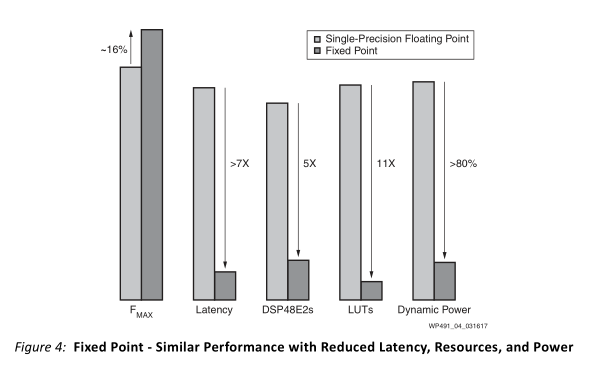
\includegraphics[height=2.5in]{figures/fp_vs_fp.png}
\\
\\
En la imagen se puede observar la diferencia en uso de recursos, tanto energéticos como de espacio entre una implementacion en punto fijo y flotante de un filtro.
Comparación de los señores de Xilinx. lo he sacado de wp491
\\\
En el caso de este proyecto, se esperaba encontrar problemas en la implementacion en el caso de que se usara punto flotante para todas las operaciones, que se materializaron en el momento de intentar sintetizar el sistema. Por tanto se procedió con la transformación del algoritmo a punto fijo.

\section{Fixed point}
Esta representación consiste de tres partes: el bit de signo, la parte entera y la parte fraccionaria. Su aritmética resulta equivalente a la de los enteros en complemento a dos.
\[1 | 0000010100001 | 01010100\]
\[signo | parte entera | parte fraccionaria\]
\\
\\
Gracias a que usa aritmética simple y el algoritmo solo necesita valores relativos y no exactos, es decir, el valor más alto encontrado en los resultados va a ser el más anómalo independientemente de si es "alto" o no, llevaron a simplificar la aritmética a enteros simples, o de punto fijo sin parte fraccionaria. (nota: estas últimas frases no me encajan muy bien).

\section{Software adaptation}
Con la intención de alcanzar el equilibrio entre resolución y uso de recursos (como visto en la tabla x) se hizo una aproximación en software. Primeramente se cambió el tipo de datos de floating point a entero de 64 bits y se observó en que pasos del algoritmo se pierde precisión por llegar a los limites representables, tanto por desbordamiento como por ser números cercanos al 0.
\\
\\
Así, si un valor se acerca a 0 será desplazado a la izquierda (multiplicado por potencias de 2) para mantener más precisión y si se encuentra cerca del desbordamiento, a la derecha, es decir, dividido, para evitarlo. Al ser los resultados relativos, no sé verán afectados siempre que estás operaciones se apliquen a todo el conjunto de datos de manera simultánea.
\\
\\
Conforme se va mejorando la precisión, también se limitan la cantidad de bits usada con el objetivo de usar menos bits en la FPGA y ahorrar lógica. Esto es de especial importancia en los DSP, donde al ser bloques definidos en fabricación, tienen operandos de tamaños fijos. Aquí se muestra una tabla con el número de DSP que necesita una multiplicación según la precisión de sus operandos.
\\
\begin{center}
 \begin{tabular}{||c c c c||} 
 \hline
 Col1 & Col2 & Col2 & Col3 \\ [0.5ex] 
 \hline\hline
 1 & 6 & 87837 & 787 \\ 
 \hline
 2 & 7 & 78 & 5415 \\
 \hline
 3 & 545 & 778 & 7507 \\
 \hline
 4 & 545 & 18744 & 7560 \\
 \hline
 5 & 88 & 788 & 6344 \\ [1ex] 
 \hline
\end{tabular}
\end{center}
Esta tabla es la tabla de bitwidth y uso de DSP

\section{Validation and precision}
->Esto estaba en el indice pero no sé si aquí debo poner otra cosa y las gráficas al final de todo en resultados. Soy consciente que tampoco ayuda que no haya hecho las gráficas y que solo haya placeholders
\\
\\
Para lograr la mayor precisión primero hay que definir esta.
Para ello se han realizado tres estrategias diferentes, en las tres tomando los resultados obtenidos por la versión en Python como la verdad.
\\
\\
Primeramente, se ha comprobado que cantidad de anomalias detectadas se pueden encontrar en las primeras x posiciones en ambos resultados, sin importar el orden.
\\
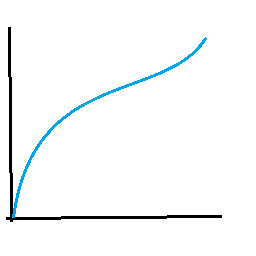
\includegraphics[height=2.5in]{figures/precision.png}
\\
\\
Ampliando la anterior estrategia, se ha comprobado para los elementos no coincidentes, si se ha detectado algun vecino en el entorno. Un vecino es definido como un pixel adyacente, tanto en linea recta como en diagonal.
\\
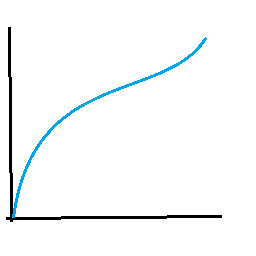
\includegraphics[height=2.5in]{figures/precision.png}
\\
\\
Para terminar se ha vuelto a extender la primera estrategia, esta vez se ha comprobado si para los no coincidentes se ha encontrado una anomalia con una similaridad espectral menor de 10 grados. (Nota: definir lo que es la similaridad espectral)
\\
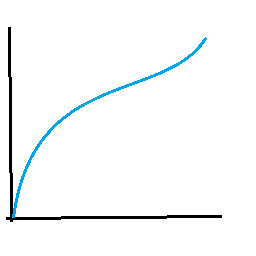
\includegraphics[height=2.5in]{figures/precision.png}
\\
\\